% !TEX root = ../Thesis.tex
\acresetall
\myChapter{Outlook}\label{ch:outlook}
\begin{flushright}{\slshape    
		So Long, and Thanks for All the Fish} \\ \medskip
    --- \defcitealias{Adams1984}{Douglas Adams}\citetalias{Adams1984} \citep{Adams1984}
\end{flushright}
\vspace{52mm}

\section{Sebastien multimodal}

\section{Structural Analysis of the lung}

\section{Skeletonization}
\todo{ATS2009-Poster, 2\textsuperscript{nd} year examination, etc.}
Multiple acinar airway skeletons have been generated from tomographic dataset as explained in my last progress report. Last year I worked on a manual method version of correcting loops and knots inside the extracted airway skeletons. Increasing both the volume of the datasets and resolution for the calculation of the airway skeletons resulted in airway descriptions containing more than \num{10000} nodes.

Figure~\ref{fig:skeleton} shows a skeletonization of multiple acini in a rat lung sample obtained at postnatal day 21 containing multiple airway segments containing one or more acini (both shown in the background). The foreground of the image shows the extracted skeletons containing between \num{1100} and \num{7300} nodes.

This big amount of skeleton points makes a manual method for correction no longer feasible. Current work on the extraction of structural information now focuses on the reproducibility of the skeleton extraction algorithm. We plan to conduct a morphological counting study for assessing the biological correctness of the computationally derived skeleton. Additionally, we started a collaboration with Fraunhofer MeVis\footnote{Which provide the visualization software MeVisLab, used for calculating the airway skeletons.} to adapt the skeletonization algorithm to segmentations obtained from our samples.

\renewcommand{\imsize}{\linewidth}
\begin{figure}[ht]
	\centering
	\pgfmathsetlength{\imagewidth}{\imsize}%
	\pgfmathsetlength{\imagescale}{\imagewidth/1541}%
	\begin{tikzpicture}[x=\imagescale,y=-\imagescale]
		%\def\x{952} % scalebar-x at golden ratio of x=1541px
		%\def\y{588} % scalebar-y at 90% of height of y=653px
		\def\x{1300} % scalebar-x at golden ratio of x=1541px
		\def\y{400} % scalebar-y at 90% of height of y=653px
		\node[anchor=north west, inner sep=0pt, outer sep=0pt] at (0,0) {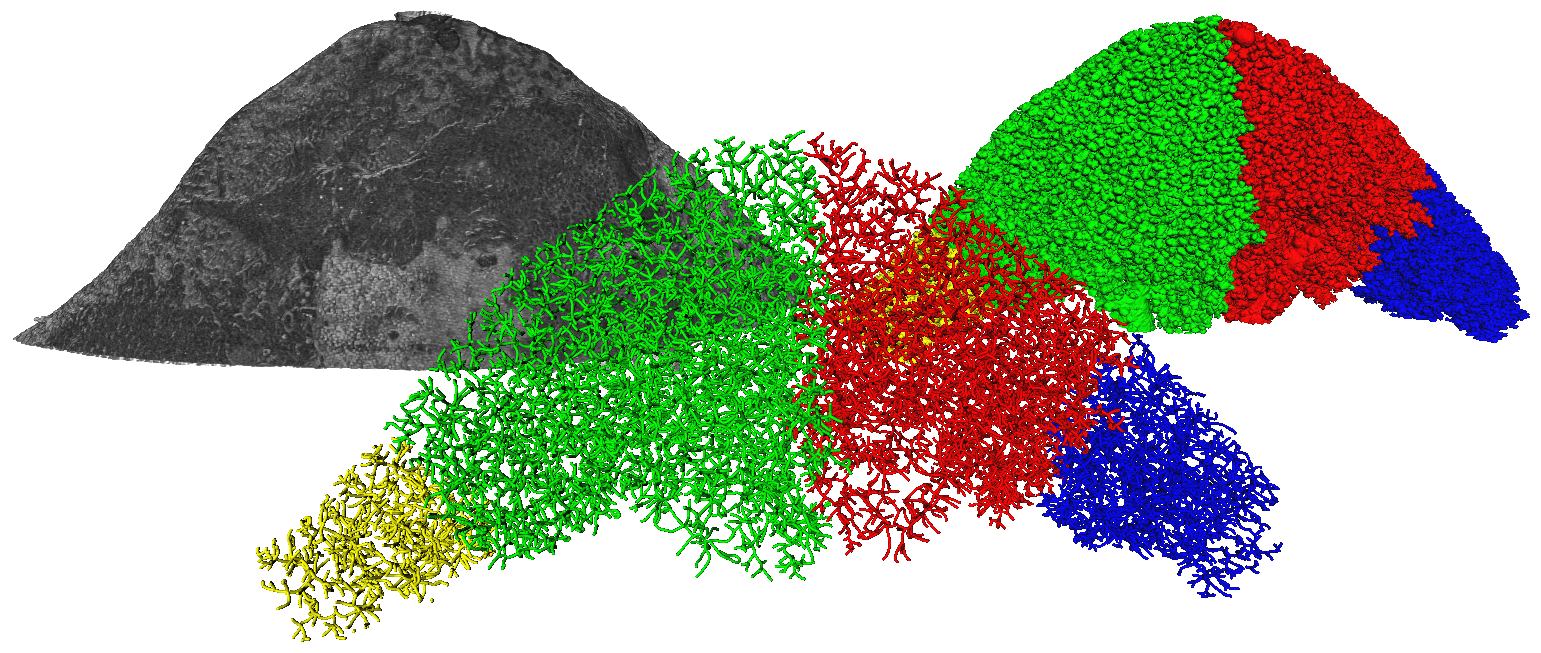
\includegraphics[width=\imagewidth]{img/R108C21b-skeleton}};
		% 796px = 4.0138mm > 100px = 504um > 99px = 500um, 20px = 100um
		%\draw[color=red,|-|,thick] (11,341) -- (807,339) node [sloped,midway,above] {\SI{4.0138}{\milli\meter} (2712px)};
		\draw[|-|,thick] (\x,\y) -- (\x+99,\y) node [midway, above] {\SI{500}{\micro\meter}};
	\end{tikzpicture}%
	\caption[\threed Visualization of rat lung sample]{Three-dimensional visualization of rat lung sample obtained at postnatal day 21. Left: Three-dimensional view of the sample, Right: Four independent airway segments. Foreground: Extracted airway skeletons of the independent airways. The yellow skeleton contains \num{1133}, the green \num{7288}, the red \num{6513} and the blue skeleton \num{3278} nodes.}
	\label{fig:skeleton}
\end{figure}

\begin{figure}
	\centering
	\renewcommand{\imsize}{\linewidth}%
	\pgfmathsetlength{\imagewidth}{\imsize}%
	\pgfmathsetlength{\imagescale}{\imagewidth/2707}%
	\subfloat[Original slice]{%
		\begin{tikzpicture}[remember picture,x=\imagescale,y=-\imagescale]%
			\node[anchor=north west, inner sep=0pt, outer sep=0pt] at (0,0) {\includegraphics[width=\imsize]{img/outlook/skeletonization/1-R108C21Cb-mrg1024}};%
      		\def\x{2300}%
			\def\y{750}%
			\draw[|-|,white,thick] (\x,\y) -- (356+\x,\y) node [midway, above] {\SI{500}{\micro\meter}};%
			\def\OLX{970} \def\OLY{356}%
			\def\URX{1504} \def\URY{820}%
			\draw[color=white, thick] (\OLX,\OLY) rectangle (\URX,\URY);%
    	\end{tikzpicture}%
		\label{subfig:skel-a}%
	}%
	\\%
	\renewcommand{\imsize}{0.5\columnwidth}%
	\subfloat[Binarized]{%
		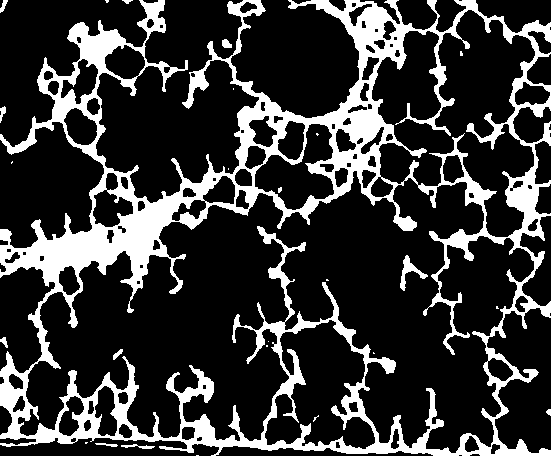
\includegraphics[width=\imsize]{img/outlook/skeletonization/4-crop-R108C21Cb-mrg1024}%
		\label{subfig:skel-b}%
		}%
	\subfloat[Segmented]{%
	 	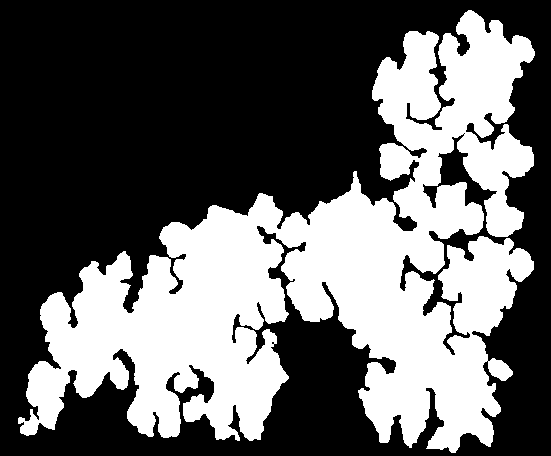
\includegraphics[width=\imsize]{img/outlook/skeletonization/5-fill-R108C21Cb-mrg1024}%
		\label{subfig:skel-c}%
		}%
	\\%
	\subfloat[Distance Transformation]{%
		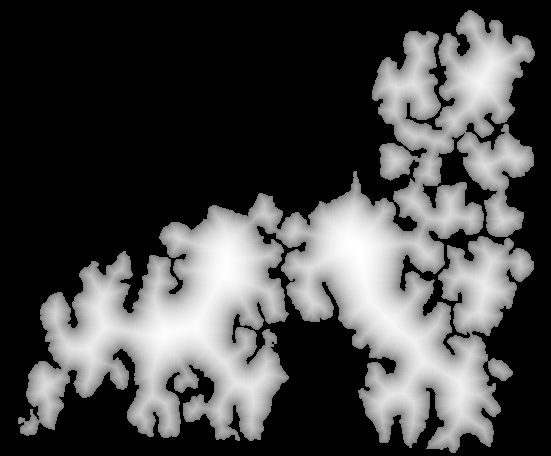
\includegraphics[width=\imsize]{img/outlook/skeletonization/6-dtf-R108C21Cb-mrg1024}%
		\label{subfig:skel-d}%
		}%
	\subfloat[Skeleton]{%
		\includegraphics[width=\imsize]{img/outlook/skeletonization/9-Skeleton-crop}%
		\label{subfig:skel-e}%
		}%
	\caption[\twod skeletonization]{Two-dimensional skeletonization process: \subref{subfig:skel-a}: Wide field scanned tomographic slice from a rat lung sample obtained at postnatal day 21. The inset corresponds to the region of the images shown in the bottom row. \subref{subfig:skel-b}: Binarized \ac{roi} The data has been separated into tissue and airspace. \subref{subfig:skel-c}: The white segment represents one connected airway structure inside the \ac{roi} in two dimensions. \subref{subfig:skel-d}: Euclidean Distance transformation of the segment shown in panel \subref{subfig:skel-c}, where the gray level value of each pixel represents the distance to the tissue-airspace border. \subref{subfig:skel-e}: The local maxima of the distance transformation form the skeleton which is then overlayed on the binarized lung structure from panel \subref{subfig:skel-a}.}%
	\label{fig:skeletonization}%
\end{figure}

\section{Acinar Growth}

\section{STEPanizer}
Explain the STEPanizer~\cite{Tschanz2010}, which has been used by Lilian and the WahlPraktikums-Students for the analyis of the \# of acini per volume.

Segmented slices (see \autoref{fig:acinus overlay} after application of ``Manhole Cover''-method with MeVisLab made the relationship of the acini visible on the twodimensional slices. This subsequently made it possible to actually count the bridges---corresponding to the alveolar entrance rings---and make a plot of the relation of the $\frac{\textrm{Acini}}{\textrm{Volume}}$ over the lung development, as shown in \autoref{fig:plot}.

\renewcommand{\imsize}{0.618\linewidth}
\begin{figure}
	\centering
	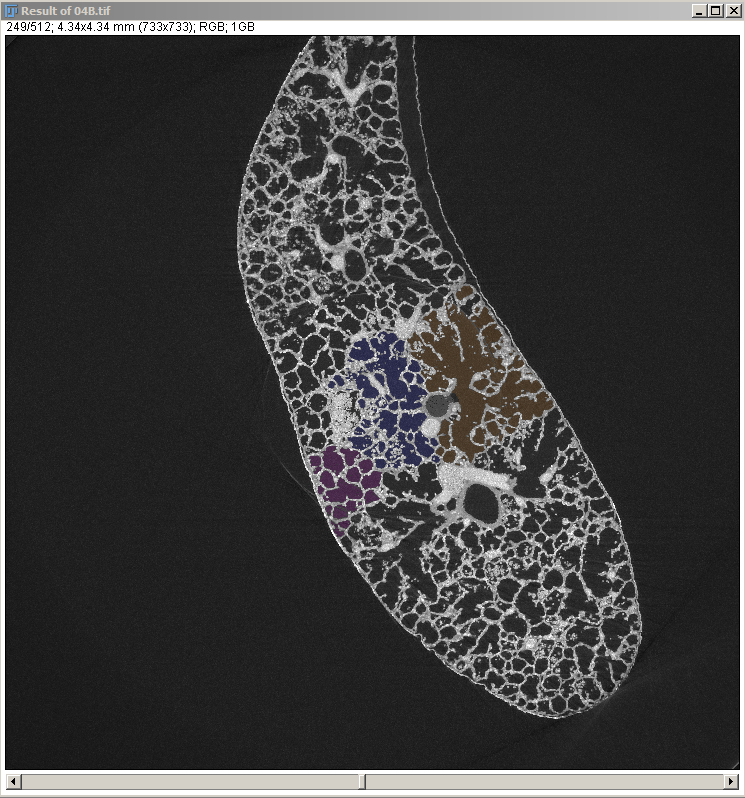
\includegraphics[width=\imsize]{img/Acinus_Overlay}
	\caption{Acinus Overlay}
	\label{fig:acinus overlay}
\end{figure}

\begin{figure}[htb]
	\noindent\makebox[\textwidth]{%
		\centering
		\begin{tikzpicture}
		\begin{axis}[
			width=\linewidth,%
			height=0.618\linewidth,%
			xmin=0,%
			xmax=60,%
			xtick={4,10,21,36,60},%
			%ytick=data,%
			xlabel=Days,%
			ylabel={Alveoli per Volume [\micro\litre$^{-1}$]}%
			]
			\addplot
				plot[error bars/.cd, y dir = both, y explicit]
				coordinates{
				 (4,830.227) +- (0,161.255)
				 (10,2068.82) +- (0,704.672)
				 (21,4257.62) +- (0,894.213)
				 (36,1406.72) +- (0,200.641)
				};
		\end{axis}
		\end{tikzpicture}%
	}
	\caption{Alveoleneingänge pro Volumen. Pro Tag wurden mehrere Segmente ausgezählt. Damit die Daten geplottet werden konnten, wurde ein Mittelwert aus diesen Segmenten gebildet. Die Fehlerbalken stellen die Standardabweichung des Mittelwerts aller gezählten Segmente dar.}
	\label{fig:plot}
\end{figure}